\documentclass{article}
\usepackage{graphicx}
\usepackage[margin=1.5cm]{geometry}
\usepackage{amsmath}

\begin{document}

\title{Thursday Reading Assessment: Unit 0, Electric Fields}
\author{Prof. Jordan C. Hanson}

\maketitle

\section{Memory Bank}

\begin{itemize}
\item $\vec{F} = q \vec{E}$ ... Force on a charge $q$ in the presence of an $\vec{E}$-field.
\item $\vec{F} = m\vec{a}$ ... Newton's 2nd Law.
\item $m = \rho V = \frac{4}{3}\pi r^3 \rho$ ... Mass of a sphere with volume $V$, density $\rho$, and radius $r$.
\end{itemize}

\section{Electric Fields}

\begin{enumerate}
\item Consider Fig. \ref{fig:ring} below.  An ink nozzle in an inkjet printer shoots microscopic ink droplets through a charging electrode, giving each droplet a charge $q$.  In the region of the deflection plates, there is an electric field $\vec{E}$ pointed upwards.  The force on the charged droplets is used to deflect them and draw a shape on the page.  Droplets without sufficient charge simply fall to the reservoir.
\begin{figure}[ht]
\centering
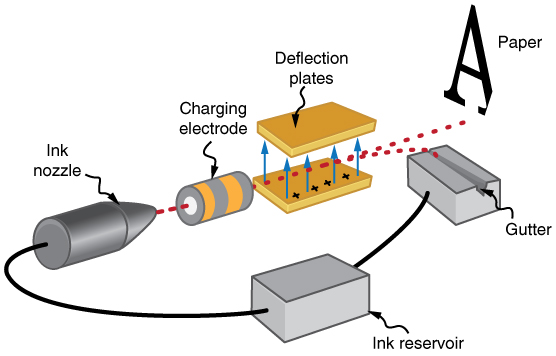
\includegraphics[width=0.4\textwidth]{inkjet.jpeg}
\caption{\label{fig:ring} A ring of charge situated in the xy-plane.}
\end{figure}
\item If the $\vec{E}$ is pointed upwards, and the $q$ on each droplet is positive, the droplets will
\begin{itemize}
\item A: Accelerate downward, if $q E$ exceeds $m g$
\item B: Accelerate upwards, if $q E$ exceeds $m g$
\item C: Travel in a straight line, if $q E$ exceeds $m g$
\item D: Fall to the reservoir
\end{itemize}
\item Suppose the the radius of the droplets is 0.1 mm, and the density of the ink is comparable to water (1 gm/cm$^3$), and $q = 1$ nC.  If $g = 9.81$ m/s$^2$, what must the value of $E$ be if the drops are to travel in a straight line?
\end{enumerate}

\end{document}
